\documentclass[conference]{IEEEtran}
\IEEEoverridecommandlockouts
\usepackage[T1]{fontenc}
\usepackage[utf8]{inputenc}
\usepackage{amsmath,amssymb}
\usepackage{graphicx}
\usepackage{booktabs}
\usepackage{multirow}
\usepackage{xcolor}
\usepackage{tikz}
\usetikzlibrary{positioning,arrows.meta,fit,calc}
\usepackage{url}
\usepackage{balance}
\usepackage[hidelinks]{hyperref}

\newcommand{\RA}{\ensuremath{\rightarrow}}
\newcommand{\best}[1]{\textbf{#1}}
% v2: every number that still has to come from the GPU run uses the red placeholder macro below.
% Before submission no placeholder may remain (see docs/GPU_RUNBOOK.md, section 5).
\newcommand{\TBD}[1]{\textcolor{red}{#1}}

\begin{document}

\title{Enhancing Cross-Modal Retrieval in Multimodal RAG through Visual-Textual Feature Fusion}

\author{\IEEEauthorblockN{Burak Efe Ko\c{c}}
\IEEEauthorblockA{\textit{Department of Computer Engineering} \\
\textit{Istanbul Technical University} \\
Istanbul, T\"urkiye \\
burakefe.koc1@gmail.com}}

\maketitle

\begin{abstract}
Multimodal retrieval-augmented generation (RAG) can only answer from the images it retrieves, so the
quality of text-to-image retrieval bounds the quality of the final answer. We build a multimodal RAG
pipeline around a unified vector database that stores, for every image, an image embedding, embeddings of
generated captions, and their fusion, and we study how visual and textual features should be combined.
On the Flickr30k 1K test set, early fusion of the image vector with a single short caption improves
text-to-image R@1 by only 0.5--2.2 points. Three changes make fusion effective: (i)~averaging the vectors of
four caption sets from BLIP and Florence-2 (+3.3 to +10.8 R@1), (ii)~scoring query--caption similarity in
a dedicated text-embedding space (BGE) and fusing it at score level (up to +14.0 over image-only
retrieval), and (iii)~a second stage that rescores the top-16 candidates with a cross-attention
image--text matching model. With a BLIP reranker the system reaches 84.9--85.9 R@1 with CLIP ViT-B/32,
CLIP ViT-L/14 and SigLIP, up from 58.8--74.6, so that after reranking the choice of dual encoder hardly
matters. A BLIP-2 reranker raises this to 88.3--88.6 R@1 for all three encoders, 1.1 points below the published
zero-shot BLIP-2 result, without any training. All weights are selected by cross-validation, and an
end-to-end evaluation of the live search code reproduces the offline numbers. On the larger and harder
MS-COCO 5K benchmark, the same pipeline with SigLIP and weights fixed on Flickr30k raises T\RA I R@1 from
46.7 (image only) to 52.2 (hybrid fusion) and to 67.3 with the BLIP-2 reranker; most of the gain again comes from the
reranker, and we analyse why the cheaper stages fall short there. Building on this analysis, a second version
of the system (v2) attacks the two remaining bottlenecks, first-stage recall and near-duplicate candidates, with
five training-free additions: region features from object detection and grid crops, detected object tags, the
contrastive (ITC) head of the BLIP-2 checkpoint as an extra first-stage channel, \emph{caption-bank hubness
normalisation} (CB-Norm), a new variant of querybank normalisation whose query bank consists of the gallery's own
generated captions and therefore needs neither training data nor test queries, and an ensemble of the three dual
encoders, followed by a joint ITM+ITC reranker over a cross-validated candidate pool. On Flickr30k 1K, v2 reaches
\TBD{XX.X} T\RA I R@1 (\TBD{+X.X} over v1, 95\% CI \TBD{[X.X, X.X]}), compared with \TBD{XX.X} for BLIP-2's own
retrieval protocol re-run in the same code and 89.7 reported in the BLIP-2 paper; on COCO 5K it reaches
\TBD{XX.X}. The retrieved images are passed to a vision-language model that answers questions
with source citations.
\end{abstract}

\begin{IEEEkeywords}
cross-modal retrieval, multimodal RAG, feature fusion, CLIP, image captioning, reranking, hubness, region features
\end{IEEEkeywords}

\section{Introduction}
Retrieval-augmented generation (RAG)~\cite{lewis2020rag} grounds a language model in documents fetched
from an external store. In multimodal RAG~\cite{chen2022murag} the store also holds images, and a user
question written in text must be matched with images. This cross-modal step is usually handled by a
dual encoder such as CLIP~\cite{radford2021clip} or SigLIP~\cite{zhai2023siglip}, which maps images and
texts into a shared embedding space where cosine similarity serves as relevance. Dual encoders are fast
and index-friendly, but they compress an image into a single vector and are known to leave a gap between
the image and text regions of the space~\cite{liang2022gap}. When the right image is not retrieved, the
generator cannot recover.

A simple remedy is to describe each image with text and use that text during retrieval: a caption lives on
the text side of the embedding space, next to the queries. This raises several design questions. How
should the image and caption representations be fused (one fused vector or a combination of scores)?
How much does caption quality matter? Is the dual encoder's text tower a good tool for comparing a query
with a caption? And how far can a more expensive cross-attention model push the result?

This project answers these questions with a complete, working system. Our contributions are:
\begin{itemize}
\item A multimodal RAG pipeline with a \emph{unified vector database} holding image, caption, text and
fused vectors under shared IDs and metadata, searchable by text, by image, or by both (Fig.~\ref{fig:arch}).
\item A controlled comparison of six fusion methods (early fusion, weighted late fusion, reciprocal rank
fusion, modality centering, multi-caption fusion and hybrid dual-encoder/text-embedding fusion) across three
dual encoders and four caption sets, with all weights chosen by cross-validation.
\item A two-stage retriever that adds cross-attention reranking and reaches 84.9--85.9 R@1 on Flickr30k 1K
for all three encoders with BLIP and 88.3--88.6 with BLIP-2, an end-to-end evaluation of the live search
code that matches the offline results, a comparison with published results under their protocols, and a
second-benchmark evaluation on MS-COCO 5K that shows where each stage helps and where it stops helping.
\item A second version (v2) with five training-free components aimed at the bottlenecks found in v1: region-level
features from detected objects and grid crops, object tags, BLIP-2 ITC as a first-stage channel, multi-encoder
ensembling, and \emph{caption-bank hubness normalisation} (CB-Norm), which corrects hub images with a bank of the
gallery's own generated captions instead of training or test queries. Every component is selected or switched off
by cross-validation, its contribution is measured in an ablation, and the final system is compared with v1 and with
BLIP-2's retrieval protocol, re-run in the same code, using paired bootstrap confidence intervals.
\end{itemize}

\section{Related Work}
\textbf{Dual encoders.} CLIP~\cite{radford2021clip} trains an image and a text encoder with a contrastive
loss on 400M image--text pairs; SigLIP~\cite{zhai2023siglip} replaces the softmax loss with a pairwise
sigmoid loss. Both produce independent embeddings that can be indexed with FAISS~\cite{johnson2019faiss}.
Liang et al.~\cite{liang2022gap} show that the two modalities occupy separate cones in the shared space
(the \emph{modality gap}), which motivates our centering experiment.

\textbf{Captioning.} BLIP~\cite{li2022blip} generates short captions; Florence-2~\cite{xiao2024florence}
is a sequence-to-sequence vision model that also produces long, detailed descriptions. Generated captions
convert visual content into text that text-only tools can use.

\textbf{Fusion.} Early fusion combines features before matching, while late fusion combines the scores
or rankings of separate matchers~\cite{snoek2005fusion}. Reciprocal rank fusion (RRF)~\cite{cormack2009rrf}
is a popular rank-level method in information retrieval.

\textbf{Cross-attention matching.} ALBEF~\cite{li2021albef} and BLIP~\cite{li2022blip} add an
image--text matching (ITM) head on top of a text transformer that cross-attends to image patch features.
These models are more accurate than dual encoders but must process every query--image pair, so they are used
for reranking.

\textbf{Region features and object tags.} Bottom-up attention~\cite{anderson2018bottomup} and
SCAN~\cite{lee2018scan} match words with detected image regions, and OSCAR~\cite{li2020oscar} feeds detected object
tags to the model as anchors between the two modalities. These methods learn the region--word alignment; our v2 uses
regions and tags without any training, through max pooling and a text-embedding channel.

\textbf{Hubness.} In high-dimensional nearest-neighbour search some items (hubs) are the nearest neighbour of
many queries~\cite{radovanovic2010hubs}. The inverted softmax~\cite{smith2017invsoftmax} and querybank
normalisation (QB-Norm)~\cite{bogolin2022qbnorm} rescale each gallery item by its similarity to a bank of
queries, which QB-Norm takes from the training set. Dual softmax~\cite{cheng2021camoe} normalises over the test
queries themselves and is therefore transductive. Our CB-Norm builds the bank from generated captions of the
gallery, so it needs neither training queries nor test queries.

\textbf{Multimodal RAG.} MuRAG~\cite{chen2022murag} retrieves images and text for open question
answering. Our work focuses on the retrieval step and shows how much it can be improved without
training any model.

\section{Method}

\begin{figure*}[t]
\centering
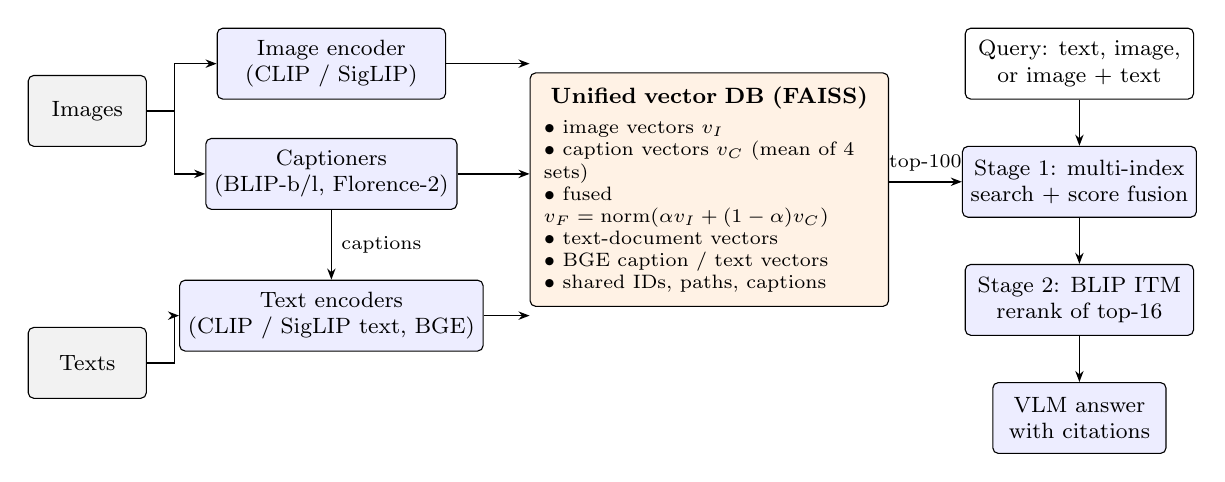
\begin{tikzpicture}[
  box/.style={draw, rounded corners=2pt, align=center, font=\footnotesize, minimum height=0.9cm,
              minimum width=2.9cm, inner sep=3pt},
  data/.style={box, fill=gray!10, minimum width=1.5cm},
  model/.style={box, fill=blue!7},
  arr/.style={-{Stealth[length=4pt]}, semithick}]
  \node[data]  (img)  at (0, 1.0)   {Images};
  \node[data]  (txt)  at (0,-2.2)   {Texts};
  \node[model] (ienc) at (3.1, 1.6) {Image encoder\\(CLIP / SigLIP)};
  \node[model] (cap)  at (3.1, 0.2) {Captioners\\(BLIP-b/l, Florence-2)};
  \node[model] (tenc) at (3.1,-1.6) {Text encoders\\(CLIP / SigLIP text, BGE)};
  \node[draw, rounded corners=2pt, fill=orange!10, text width=4.2cm, align=left, font=\scriptsize,
        inner sep=5pt] (db) at (7.9, 0) {%
    \centering{\footnotesize\bfseries Unified vector DB (FAISS)}\par\vspace{3pt}
    \raggedright
    $\bullet$ image vectors $v_I$\\
    $\bullet$ caption vectors $v_C$ (mean of 4 sets)\\
    $\bullet$ fused $v_F=\mathrm{norm}(\alpha v_I+(1-\alpha)v_C)$\\
    $\bullet$ text-document vectors\\
    $\bullet$ BGE caption / text vectors\\
    $\bullet$ shared IDs, paths, captions};
  \node[box]   (query) at (12.6, 1.6)  {Query: text, image,\\or image + text};
  \node[model] (s1)    at (12.6, 0.1)  {Stage 1: multi-index\\search + score fusion};
  \node[model] (s2)    at (12.6,-1.4)  {Stage 2: BLIP ITM\\rerank of top-16};
  \node[model, minimum width=2.2cm] (gen) at (12.6,-2.9) {VLM answer\\with citations};
  \draw[arr] (img.east) -- ++(0.35,0) |- (ienc.west);
  \draw[arr] (img.east) -- ++(0.35,0) |- (cap.west);
  \draw[arr] (txt.east) -- ++(0.35,0) |- (tenc.west);
  \draw[arr] (cap.south) -- node[right, font=\scriptsize] {captions} (tenc.north);
  \draw[arr] (ienc.east) -- (ienc.east -| db.west);
  \draw[arr] (cap.east)  -- (cap.east -| db.west);
  \draw[arr] (tenc.east) -- (tenc.east -| db.west);
  \draw[arr] (query) -- (s1);
  \draw[arr] (db.east |- s1.west) -- node[above, font=\scriptsize] {top-100} (s1.west);
  \draw[arr] (s1) -- (s2);
  \draw[arr] (s2) -- (gen);
\end{tikzpicture}
\caption{System overview. Images and texts are encoded into a unified vector database. A query is matched
against several indexes, the score lists are fused (stage~1), the top-16 images are rescored with a
cross-attention ITM model (stage~2), and the results are passed to a vision-language model.}
\label{fig:arch}
\end{figure*}

\subsection{Unified Vector Database}
Every item (image or text document) has an ID, a path or text, and metadata. For an image item we store
the image embedding $v_I = E_I(x)$ from the dual encoder and the embeddings of its generated captions
$c_1,\dots,c_m$. Text documents get a text embedding $v_T$. All vectors are $\ell_2$-normalised and kept
in one exact inner-product FAISS index per vector type. Raw vectors are saved, so fused indexes for a new
$\alpha$ or with centering can be rebuilt without running any network.

\subsection{Visual-Textual Fusion}
\textbf{Early fusion.} A fused document vector mixes the image and caption vectors:
\begin{equation}
\begin{aligned}
v_F &= \mathrm{norm}\big(\alpha\, v_I + (1-\alpha)\, v_C\big),\\
v_C &= \mathrm{norm}\Big(\tfrac{1}{m}\textstyle\sum_{j=1}^{m} E_T(c_j)\Big),
\end{aligned}
\label{eq:early}
\end{equation}
where $E_T$ is the dual encoder's text tower. With $m=1$ this is standard image--caption fusion; with
$m>1$ (\emph{multi-caption}) several caption sets are averaged, which reduces the noise of any single
caption. A text query $q$ is scored by $\langle E_T(q), v_F\rangle$.

\textbf{Late fusion.} Scores of the image and caption indexes are fused after retrieval. Because raw
cosine scores of different modality pairs lie on different scales, we z-normalise each score list per
query and take a weighted sum, $s = \sum_k w_k\, z(s_k)$. We also test RRF~\cite{cormack2009rrf},
$s(d)=\sum_k 1/(60 + \mathrm{rank}_k(d))$, which ignores score magnitudes.

\textbf{Modality centering.} To reduce the modality gap~\cite{liang2022gap} we subtract the mean image
vector from image vectors and the mean text-side vector from caption and query vectors, then
re-normalise.

\textbf{Hybrid fusion with a text embedder.} The CLIP/SigLIP text tower is trained to match images, not to
compare two sentences, and it truncates input at 77 (CLIP) or 64 tokens. We therefore embed the query and
the captions a second time with a dedicated sentence-embedding model, BGE-base~\cite{xiao2023bge}
(inputs of up to 256 tokens in our setup), and fuse at score level:
\begin{equation}
s(q,d) = (1-w)\, z\big(\langle E_T(q), v_F\rangle\big) + w\, z\big(\langle B(q), B(c_{1:m})\rangle\big),
\label{eq:hybrid}
\end{equation}
where $B$ is BGE and $c_{1:m}$ is the concatenation of all caption sets of the image.

\textbf{Query fusion.} For an image + text query the two query embeddings are mixed the same way,
$q = \mathrm{norm}(\beta\, E_I(x_q) + (1-\beta)\, E_T(t_q))$, so a user can ask for ``this image, but
at night''.

\subsection{Two-Stage Retrieval with Cross-Attention Reranking}
Stage~1 retrieves the top-100 candidates from each index and fuses them. Stage~2 rescores the top-$K=16$
images with the ITM head of BLIP~\cite{li2022blip} (fine-tuned on COCO~\cite{lin2014coco}): the query is
encoded by a text transformer that cross-attends to the image patch features, and the head outputs
$p_\mathrm{ITM} = P(\text{match}\mid q, x)$. This is the most fine-grained form of visual-textual
fusion in the system. The final score is
$\lambda\, z(p_\mathrm{ITM}) + (1-\lambda)\, z(s_\mathrm{stage1})$ over the $K$ candidates. The patch
features of each image are computed once and cached, so each extra query--image pair costs only one pass
of the text transformer.

We also test a stronger cross-encoder, the ITM head of BLIP-2~\cite{li2023blip2} (frozen ViT-g image
encoder, fine-tuned on COCO). In BLIP-2, 32 learned query tokens and the text tokens attend to each other
inside a Q-Former that cross-attends to the ViT-g patch features; the ITM logits are averaged over the
query tokens. We cache the ViT-g features in the same way, and check that the cached path gives the same
probabilities as the reference implementation. The two ITM scores can also be combined,
$a\, z(p_\mathrm{BLIP}) + b\, z(p_\mathrm{BLIP\text{-}2}) + (1-a-b)\, z(s_\mathrm{stage1})$.

\subsection{Version 2: Beyond One Global Vector}
\label{sec:v2}
The v1 results (Section~\ref{sec:results}) leave two bottlenecks: candidates the first stage misses cannot be
recovered by the reranker (recall@16 is 97.4--98.1 on Flickr30k and at least 87.8 on COCO), and the cheap
channels cannot separate near-duplicate scenes, because a global vector and a caption both describe the gist of
an image. v2 adds the following training-free components. All of them are cached at indexing time.

\textbf{Region features.} For each image $g$ we form a region set $\mathcal{R}_g$: four overlapping quadrant
crops (60\% of each side), a 70\% centre crop, and up to six object boxes from Florence-2~\cite{xiao2024florence}
\texttt{<OD>} (largest first, area between 2\% and 90\% of the image, 10\% context margin, near-duplicates with
IoU $>0.8$ removed). Every crop is encoded by the dual encoder's image tower, and an image is scored by its
best-matching region,
\begin{equation}
s_\mathrm{reg}(q,g)=\max_{r\in\mathcal{R}_g}\langle E_T(q), E_I(x_r)\rangle .
\label{eq:region}
\end{equation}
Max pooling acts as a hard, untrained attention: a query about a small object can match the crop that
contains it, which a 224-pixel global view may blur.

\textbf{Object tags.} The labels of the kept boxes form a short text (``dog, frisbee, grass''), embedded with
BGE; $s_\mathrm{tag}(q,g)=\langle B(q), B(\mathrm{tags}_g)\rangle$. Tags name objects that a caption may omit.

\textbf{BLIP-2 ITC channel.} The BLIP-2 reranker checkpoint also contains a contrastive head: the Q-Former turns
an image into 32 query embeddings $z_{g,1..32}$ and a text into one embedding $t_q$, and
$s_\mathrm{itc}(q,g)=\max_k \langle t_q, z_{g,k}\rangle$. The image side is precomputed, so this channel costs one
text encoding per query, and its errors differ from those of CLIP/SigLIP, which should raise the recall of the
candidate pool. We verified that our cached computation reproduces
\texttt{Blip2ForImageTextRetrieval} exactly.

\textbf{Greedy stage-1 combination.} Channels are added one at a time to the hybrid score of
Eq.~(\ref{eq:hybrid}): $s^{(k)}=(1-\gamma_k)\,z(s^{(k-1)})+\gamma_k\, z(s_k)$, with
$\gamma_k\in\{0,0.1,\dots,1\}$ chosen by cross-validation, so CV can switch a channel off ($\gamma_k=0$).

\textbf{Caption-bank hubness normalisation (CB-Norm).} Hub images are close to many queries and take rank~1
from the correct image. QB-Norm~\cite{bogolin2022qbnorm} detects them with a bank of training queries. We
instead use the captions that BLIP-base and BLIP-large generated for the gallery images ($2N$ pseudo-queries
$\mathcal{B}$, each owned by one image). For a channel $c$ and gallery item $g$,
\begin{equation}
\begin{aligned}
L^c_g &= \log \frac{1}{|\mathcal{B}_{\neg g}|}\sum_{b\in\mathcal{B}_{\neg g}} \exp\big(\beta\, s^c(b,g)\big),\\
\tilde{s}^c(q,g) &= s^c(q,g) - \tfrac{\rho}{\beta}\big(L^c_g-\bar{L}^c\big),
\end{aligned}
\label{eq:cbnorm}
\end{equation}
where $\mathcal{B}_{\neg g}$ excludes the captions of $g$ itself (otherwise an image with good captions would
be penalised for them) and $\bar{L}^c$ is the mean over the gallery. With $\rho=1$ this is the inverted
softmax~\cite{smith2017invsoftmax} over the bank; $\rho=0$ switches it off. $L^c_g$ is computed once per item,
so the query-time cost is one subtraction per score. Unlike dual softmax~\cite{cheng2021camoe}, CB-Norm never
looks at the test queries, and unlike QB-Norm it needs no training split. We apply it to every channel with a
shared $(\beta,\rho)\in\{10,20,50\}\times\{0,0.25,0.5,0.75,1\}$ chosen by CV.

\textbf{Encoder ensemble.} The final stage-1 scores of CLIP ViT-B/32, CLIP ViT-L/14 and SigLIP are
z-normalised and averaged with equal weights (no tuning).

\textbf{Stage 2 with ITM and ITC.} Over the top-$K$ candidates the final score is
\begin{equation}
s = \lambda_1 z(p_\mathrm{ITM}) + \lambda_2 z(s_\mathrm{itc}) + (1-\lambda_1-\lambda_2)\, z(s_1),
\label{eq:rerank2}
\end{equation}
where $(K,\lambda_1,\lambda_2)$ with $K\in\{16,32,64\}$ and $\lambda_1+\lambda_2\le 1$ is chosen by CV, so a
larger pool is used only if it helps on held-out queries. For reference we also re-run BLIP-2's own retrieval
protocol~\cite{li2023blip2} in our code: ITC top-128, then ITM logit plus ITC similarity.

\subsection{Answer Generation}
The top results (images with their captions, and text documents) are sent to a vision-language model
(Claude Opus~5.5\footnote{Model ID \texttt{claude-opus-5-5}, accessed through the Anthropic API.}) with an
instruction to answer only from the provided sources and to cite them as [S1], [S2],~\dots

\section{Experimental Setup}
\textbf{Data.} We use the standard Flickr30k~\cite{young2014flickr} 1K test split~\cite{karpathy2015deep}:
1000 images with 5 human captions each, giving 5000 text queries for text\RA image (T\RA I) retrieval
and 1000 image queries for image\RA text (I\RA T) retrieval. The human captions are used only as queries
and ground truth, never as image metadata. As a second benchmark we use the MS-COCO~\cite{lin2014coco} 2014
5K test split: 5000 images and 25{,}010 captions (a few images have more than five), used the same way. For
COCO we evaluate 1000 randomly sampled text queries (fixed seed) through the live search path with SigLIP only.

\textbf{Models.} Dual encoders: CLIP ViT-B/32, CLIP ViT-L/14 and SigLIP-base (patch 16, 224px). Caption
sets: BLIP-base (blip-b), BLIP-large (blip-l), and Florence-2-large with the
\texttt{<DETAILED\_CAPTION>} (flor-d) and \texttt{<MORE\_DETAILED\_CAPTION>} (flor-md) tasks, averaging
7.1, 12.9, 44.8 and 90.6 words per caption. Text embedder: BGE-base-en-v1.5. Rerankers:
BLIP ITM base and BLIP-2 ITM ViT-g, both fine-tuned on COCO and never on Flickr30k. No model is trained
or fine-tuned by us.

\textbf{Metrics.} Recall at $k$ (R@1, R@5, R@10), the sum RSUM, and mean reciprocal rank (MRR).

\textbf{Weight selection.} The images are split into two random folds. Every weight ($\alpha$, $w$,
$\lambda$) is chosen on one fold by RSUM and applied to queries of the other fold, so no query is
evaluated with a weight tuned on it. The reported numbers are therefore fair estimates for unseen data,
not oracle values. In v2 the components are added greedily: each new weight is chosen on the same folds with the
earlier weights fixed, and every grid contains the value that switches the component off.

\textbf{Significance.} For the v2 system we report the difference in R@1 to the v1 system and to the re-run
BLIP-2 protocol with a 95\% paired bootstrap confidence interval over queries (2000
resamples)~\cite{efron1993bootstrap}. The v2 system that is tested (the encoder ensemble with ITM+ITC reranking) is
fixed in advance, not chosen as the best row on the test set.

\textbf{Implementation.} PyTorch, HuggingFace Transformers and FAISS on a single RTX~5070 GPU, run in a
throttled ``quiet'' mode (a short pause after every batch). Captions are generated once per image and
cached, and are shared by all encoders.

\section{Results}
\label{sec:results}

\subsection{Fusion with a Single Short Caption}
Table~\ref{tab:part1} compares fusion methods with BLIP-base captions. Early fusion beats image-only
retrieval for every encoder, but the gain is small (+2.2, +1.3 and +0.5 R@1) and shrinks as the encoder gets
stronger. Captions alone are weak (22--25 R@1): seven-word BLIP captions are generic (``two dogs playing
in the snow'') and many test images share them. Weighted late fusion with z-normalised scores performs about
as well as early fusion. Equal-weight RRF is harmful (about 40 R@1): it gives the weak caption ranking the
same vote as the image ranking. Score-level fusion only works when weighted. Modality centering helps CLIP
slightly but hurts SigLIP by 2.4--2.7 points, and it hurts I\RA T retrieval for all encoders (4.4--7.2 R@1),
so it is off by default.

Fig.~\ref{fig:alpha} shows the effect of $\alpha$. Performance peaks at $\alpha=0.90$--$0.96$: a small
amount of caption information helps, but the image vector must dominate. The stronger the encoder, the
higher the best $\alpha$.

\begin{table}[t]
\centering
\caption{T\RA I R@1 on Flickr30k 1K with BLIP-base captions.}
\label{tab:part1}
\setlength{\tabcolsep}{5pt}
\begin{tabular}{lccc}
\toprule
Method & CLIP B/32 & CLIP L/14 & SigLIP \\
\midrule
Image only            & 58.76 & 64.58 & 74.58 \\
Caption only          & 24.64 & 24.68 & 21.94 \\
Early fusion          & \best{60.98} & 65.88 & 75.10 \\
Late fusion (z-score) & 60.26 & 65.48 & \best{75.24} \\
RRF (equal weights)   & 39.92 & 40.18 & 38.98 \\
Image only + centering   & 60.14 & 66.78 & 72.18 \\
Early fusion + centering & 60.96 & \best{67.16} & 72.38 \\
\bottomrule
\end{tabular}
\end{table}

\begin{figure}[t]
\centering
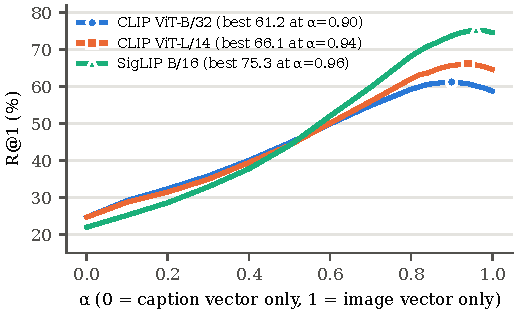
\includegraphics[width=\columnwidth]{figures/alpha_sweep.pdf}
\caption{T\RA I R@1 versus the early-fusion weight $\alpha$ (BLIP-base captions, full test set). The
marker shows the best $\alpha$ of each encoder.}
\label{fig:alpha}
\end{figure}

\subsection{Better Captions, Multi-Caption and Hybrid Fusion}
Table~\ref{tab:part2} reports the improvements. Three findings stand out.

\emph{Caption quality is the main lever.} Replacing BLIP-base with BLIP-large or the detailed Florence-2
captions raises early fusion on CLIP ViT-L/14 from 65.9 to 71.3 R@1. Averaging the four caption sets
(Eq.~\ref{eq:early}, $m=4$) helps further, reaching 69.5, 73.0 and 77.9 R@1 (+10.8, +8.4 and +3.3 over
image-only). Different captioners make different mistakes, and averaging their vectors cancels part of them.

\emph{A text model should compare text with text.} In BGE space, the most detailed Florence-2 captions alone
reach 60.8 R@1 without looking at the image vector at all, more than CLIP ViT-B/32 image retrieval (58.8)
and far above CLIP's own text tower on captions (about 25). BGE handles long captions that CLIP truncates.
The concatenation of all four caption sets gives 63.2.

\emph{The channels are complementary.} The hybrid score (Eq.~\ref{eq:hybrid}) beats both of its parts for
every encoder: 72.8, 75.6 and 78.8 R@1. This also improves SigLIP, for which single-caption early fusion
barely helped. The selected text weight $w$ is 0.2--0.4.

\begin{table*}[t]
\centering
\caption{T\RA I retrieval on Flickr30k 1K (5000 queries). All weights are chosen by 2-fold cross-validation
over images. The te-caption rows use only BGE caption embeddings and do not depend on the dual encoder.}
\label{tab:part2}
\setlength{\tabcolsep}{4.5pt}
\begin{tabular}{l ccc ccc ccc}
\toprule
& \multicolumn{3}{c}{CLIP ViT-B/32} & \multicolumn{3}{c}{CLIP ViT-L/14} & \multicolumn{3}{c}{SigLIP-base} \\
\cmidrule(lr){2-4}\cmidrule(lr){5-7}\cmidrule(lr){8-10}
Method & R@1 & R@5 & R@10 & R@1 & R@5 & R@10 & R@1 & R@5 & R@10 \\
\midrule
Image only                   & 58.76 & 83.44 & 90.08 & 64.58 & 87.06 & 92.16 & 74.58 & 92.30 & 95.64 \\
\midrule
Early fusion, blip-b         & 61.16 & 84.48 & 90.72 & 65.88 & 88.44 & 93.16 & 74.64 & 92.22 & 95.64 \\
Early fusion, blip-l         & 64.24 & 86.30 & 92.18 & 67.62 & 89.06 & 93.70 & 75.40 & 92.84 & 96.08 \\
Early fusion, flor-d         & 62.84 & 85.88 & 91.78 & 69.52 & 90.58 & 94.78 & 76.28 & 92.76 & 95.98 \\
Early fusion, flor-md        & 63.54 & 86.80 & 92.26 & 71.32 & 90.86 & 94.86 & 76.44 & 92.98 & 96.10 \\
Early fusion, multi-caption  & 69.54 & 89.56 & 93.96 & 72.96 & 92.10 & 95.52 & 77.92 & 93.70 & 96.62 \\
\midrule
te-caption (BGE), flor-md    & 60.82 & 84.42 & 90.12 & 60.82 & 84.42 & 90.12 & 60.82 & 84.42 & 90.12 \\
te-caption (BGE), concat     & 63.18 & 85.62 & 91.12 & 63.18 & 85.62 & 91.12 & 63.18 & 85.62 & 91.12 \\
Hybrid, flor-md              & 70.84 & 91.68 & 95.38 & 74.88 & 92.82 & 96.06 & 78.48 & 94.24 & 96.80 \\
Hybrid, multi-caption        & 72.78 & 92.18 & 95.84 & 75.64 & 93.62 & 96.78 & 78.78 & 94.18 & 97.00 \\
\midrule
Hybrid + ITM rerank (top-16) & \best{84.92} & \best{96.08} & \best{97.18} & \best{85.92} & \best{96.70} & \best{97.82} & \best{85.50} & \best{96.76} & \best{97.74} \\
\bottomrule
\end{tabular}
\end{table*}

\subsection{Cross-Attention Reranking}
Reranking the top-16 hybrid candidates with BLIP ITM gives the largest jump: 84.9, 85.9 and 85.5 R@1
(Table~\ref{tab:part2}, last row), +26.2, +21.3 and +10.9 over image-only retrieval. It works because the
fused first stage places the correct image in the top-16 for 97.4\%, 98.1\% and 98.0\% of queries; this
recall is the upper bound of stage~2. After reranking the three encoders are within one point of each
other, so the job of the first stage changes from ranking precisely to reaching high recall@16 cheaply.
The selected $\lambda$ is 0.7--0.9, so the ITM score dominates; using the ITM score alone ($\lambda=1$)
gives similar results (85.2--85.4 R@1), which shows that most of the stage-2 gain comes from the
cross-attention model. Fig.~\ref{fig:stages} summarises the contribution of each component.

\begin{figure}[t]
\centering
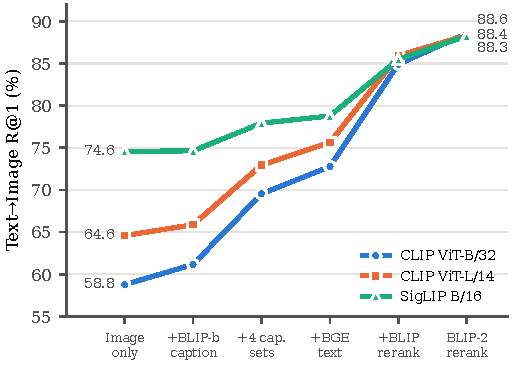
\includegraphics[width=\columnwidth]{figures/stages.pdf}
\caption{T\RA I R@1 as components are added (Flickr30k 1K, cross-validated weights). The last point
replaces the BLIP reranker with BLIP-2.}
\label{fig:stages}
\end{figure}

\subsection{A Stronger Cross-Encoder: BLIP-2}
Table~\ref{tab:blip2} replaces the BLIP reranker with BLIP-2 on the same top-16 candidates. R@1 rises
by a further 3.7 points for CLIP ViT-B/32 (84.9\RA 88.6), 2.4 for ViT-L/14 (85.9\RA 88.4) and 2.8 for
SigLIP (85.5\RA 88.3), so all three encoders again end within 0.3 points of each other. The
cross-validated $\lambda$ is 0.9--1.0, so BLIP-2 needs almost no help from the first-stage score. Adding the
BLIP score on top of BLIP-2 does not help further (88.2, 88.7 and 88.4, within noise of BLIP-2 alone): the
weaker cross-encoder adds little that the stronger one misses. The remaining errors are bounded by the first
stage, which misses the correct image in 1.9--2.6\% of the queries (recall@16 97.4--98.1). When the
correct image \emph{is} in the top-16, BLIP-2 ranks it first about 90\% of the time. R@5 and R@10 change
much less than R@1, because they are already close to recall@16.

\begin{table}[t]
\centering
\caption{T\RA I R@1 / R@5 on Flickr30k 1K: reranking the hybrid top-16 with BLIP vs.\ BLIP-2 ITM
(cross-validated weights).}
\label{tab:blip2}
\setlength{\tabcolsep}{3.4pt}
\begin{tabular}{l cc cc cc}
\toprule
& \multicolumn{2}{c}{CLIP B/32} & \multicolumn{2}{c}{CLIP L/14} & \multicolumn{2}{c}{SigLIP} \\
\cmidrule(lr){2-3}\cmidrule(lr){4-5}\cmidrule(lr){6-7}
Stage 2 & R@1 & R@5 & R@1 & R@5 & R@1 & R@5 \\
\midrule
none (hybrid)        & 72.78 & 92.18 & 75.64 & 93.62 & 78.78 & 94.18 \\
BLIP ITM             & 84.92 & 96.08 & 85.92 & 96.70 & 85.50 & 96.76 \\
BLIP-2 ITM           & \best{88.58} & 96.62 & 88.36 & \best{97.40} & 88.28 & \best{97.32} \\
BLIP + BLIP-2        & 88.24 & \best{96.72} & \best{88.68} & \best{97.40} & \best{88.36} & \best{97.32} \\
\midrule
recall@16 (bound)    & \multicolumn{2}{c}{97.36} & \multicolumn{2}{c}{98.06} & \multicolumn{2}{c}{98.02} \\
\bottomrule
\end{tabular}
\end{table}

\subsection{Version 2: Components, Ablations and Final System}
\label{sec:v2res}
% TODO(GPU run): fill every \TBD{} from results/tables/flickr1k_v2.md (rows are named as in the table below), then
% rewrite the prose of this subsection to match the numbers. Keep a sentence only if the numbers support it; if CV
% switched a component off (picked weight 0 in both folds), say so plainly.
Table~\ref{tab:v2chain} adds the v2 components one at a time to the v1 hybrid first stage of each encoder;
Table~\ref{tab:v2abl} isolates them, and Table~\ref{tab:v2final} compares the complete system with v1 and with
BLIP-2's retrieval protocol re-run in our code.

\begin{table}[t]
\centering
\caption{v2 stage-1 chain, T\RA I R@1 on Flickr30k 1K (5000 queries, 2-fold CV over images). Each row adds one
component to the row above; ``rec@64'' is the share of queries whose image is in the top-64.}
\label{tab:v2chain}
\setlength{\tabcolsep}{4pt}
\begin{tabular}{lccc}
\toprule
Stage 1 & CLIP B/32 & CLIP L/14 & SigLIP \\
\midrule
Image only                     & 58.76 & 64.58 & 74.58 \\
Hybrid, multi-caption (v1)     & 72.78 & 75.64 & 78.78 \\
+ object tags (BGE) & \TBD{--} & \TBD{--} & \TBD{--} \\
+ region features & \TBD{--} & \TBD{--} & \TBD{--} \\
+ BLIP-2 ITC channel & \TBD{--} & \TBD{--} & \TBD{--} \\
+ CB-Norm & \TBD{--} & \TBD{--} & \TBD{--} \\
\midrule
Ensemble of the three          & \multicolumn{3}{c}{\TBD{--}} \\
rec@16 / rec@64 (ensemble)     & \multicolumn{3}{c}{\TBD{--} / \TBD{--}} \\
\bottomrule
\end{tabular}
\end{table}

\begin{table}[t]
\centering
\caption{Ablations on Flickr30k 1K, T\RA I R@1. Each row adds a single component to the v1 hybrid score of the
same encoder (not chained), or scores with one channel alone. $\ddagger$: transductive, uses all test queries at
once; not comparable and not part of our system.}
\label{tab:v2abl}
\setlength{\tabcolsep}{4pt}
\begin{tabular}{lccc}
\toprule
Variant & CLIP B/32 & CLIP L/14 & SigLIP \\
\midrule
Hybrid (v1)                         & 72.78 & 75.64 & 78.78 \\
+ grid crops only & \TBD{--} & \TBD{--} & \TBD{--} \\
+ detected-object crops only & \TBD{--} & \TBD{--} & \TBD{--} \\
+ BLIP-2 ITC only & \TBD{--} & \TBD{--} & \TBD{--} \\
\midrule
BGE object tags alone               & \multicolumn{3}{c}{\TBD{--}} \\
BLIP-2 ITC alone (full gallery)     & \multicolumn{3}{c}{\TBD{--}} \\
Ensemble + dual softmax$^\ddagger$  & \multicolumn{3}{c}{\TBD{--}} \\
\bottomrule
\end{tabular}
\end{table}

\begin{table}[t]
\centering
\caption{Final systems on Flickr30k 1K (5000 queries). All rows run in our code with the BLIP-2 ITM ViT-g
checkpoint. $\Delta$: R@1 gain of v2 with a 95\% paired bootstrap CI.}
\label{tab:v2final}
\setlength{\tabcolsep}{3pt}
\begin{tabular}{l ccc c}
\toprule
System & R@1 & R@5 & R@10 & $\Delta$R@1 of v2 [CI] \\
\midrule
BLIP-2 protocol, re-run (ITC top-128)  & \TBD{--} & \TBD{--} & \TBD{--} & \TBD{+X.X [X.X, X.X]} \\
v1: B/32 hybrid + BLIP-2 (top-16)      & \TBD{88.58} & \TBD{--} & \TBD{--} & \TBD{+X.X [X.X, X.X]} \\
v2: ensemble + ITM+ITC (CV $K$)        & \best{\TBD{--}} & \TBD{--} & \TBD{--} & -- \\
\bottomrule
\end{tabular}
\end{table}

% TODO(GPU run): one paragraph per question, numbers from the tables above:
% (1) Which channels did CV keep, with which weights (results/json/flickr1k_v2.json, "picked")? Which helped most?
% (2) Regions: grid vs. detected objects -- does object-level evidence help more than fixed crops?
% (3) BLIP-2 ITC: how much does it raise recall@16/@64, i.e. the upper bound of stage 2?
% (4) CB-Norm: does it help, which (beta, rho) did CV pick, and is the gain larger for the weaker encoders?
% (5) Final: is v2 above v1 and above the re-run BLIP-2 protocol with a CI that excludes 0? Which K did CV pick?
\TBD{Results discussion to be written from the GPU run.}

% TODO(GPU run): uncomment once scripts/make_figures.py has written report/figures/v2_stages_flickr1k.pdf
% \begin{figure}[t]
% \centering
% 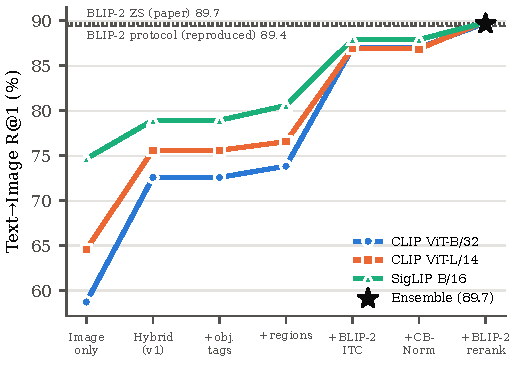
\includegraphics[width=\columnwidth]{figures/v2_stages_flickr1k.pdf}
% \caption{T\RA I R@1 along the v2 chain on Flickr30k 1K. Dotted: BLIP-2 zero-shot as published; dashed: BLIP-2
% protocol re-run in our code. Star: encoder ensemble with ITM+ITC reranking.}
% \label{fig:v2stages}
% \end{figure}

\subsection{Comparison with Published Results}
Table~\ref{tab:published} places our system next to published Flickr30k 1K results. The numbers are copied
from the original papers. Protocols differ, so the table is a reference point and not a leaderboard. Three
groups are relevant:
\begin{itemize}
\item \emph{Zero-shot dual encoders} (CLIP, ALIGN) are not trained on any retrieval data. Our full system
is about 13 R@1 points above the best of them, but this comparison favours us: our rerankers were
fine-tuned on COCO, whereas CLIP and ALIGN saw no retrieval training data at all. Our own CLIP ViT-L/14
image-only result (64.6) is lower than the published 68.7 because the paper uses 336\,px inputs and a
``a photo of'' prompt.
\item \emph{COCO-fine-tuned models transferred to Flickr30k} (ALBEF, BLIP, BLIP-2) use the same protocol as
our rerankers: fine-tuned on COCO, evaluated on Flickr30k without further training, with an ITM rerank of
the top-$k$ candidates of their own dual encoder ($k=128$ for BLIP and BLIP-2). Our results are in this
range: 88.6 R@1 with BLIP-2, 1.1 points below the published BLIP-2 ViT-g result (89.7) although our
first stage is a frozen CLIP ViT-B/32 with captions instead of BLIP-2's own fine-tuned features, and we
rerank only $k=16$ candidates.
\item \emph{Models fine-tuned on Flickr30k} use its 29K training images. BEiT-3 (90.3) remains ahead.
\end{itemize}
Our R@5 and R@10 are lower than those of the reranked baselines because only 16 candidates are rescored,
which caps both near recall@16 (97.4--98.1); a larger $k$ would raise them at higher cost. In short, the
system does not set a new state of the art, but it shows that combining frozen, off-the-shelf models with
fusion reaches the level of task-specific vision-language models without any training.
% TODO(GPU run): update this paragraph with the v2 row. Claim "above BLIP-2 zero-shot (89.7)" or "state of the art
% among zero-shot methods" ONLY if the v2 R@1 and the lower end of its CI against the re-run protocol support it,
% and keep the protocol caveats (COCO-fine-tuned reranker; BEiT-3 is fine-tuned on Flickr30k).

\begin{table}[t]
\centering
\caption{T\RA I on Flickr30k 1K: published results (numbers from the cited papers) and ours. ZS: no
Flickr30k training; ``COCO'' marks models fine-tuned on COCO; FT: fine-tuned on Flickr30k. $\dagger$: with
ITM reranking of the top-$k$.}
\label{tab:published}
\setlength{\tabcolsep}{3.5pt}
\begin{tabular}{l l ccc}
\toprule
Method & Protocol & R@1 & R@5 & R@10 \\
\midrule
CLIP ViT-L/14@336~\cite{radford2021clip}  & ZS          & 68.7 & 90.6 & 95.2 \\
ALIGN~\cite{jia2021align}                 & ZS          & 75.7 & 93.8 & 96.8 \\
\midrule
ALBEF 14M$^\dagger$~\cite{li2021albef}    & ZS, COCO    & 82.8 & 96.3 & 98.1 \\
BLIP ViT-L$^\dagger$~\cite{li2022blip}    & ZS, COCO    & 86.7 & 97.3 & 98.7 \\
BLIP-2 ViT-g$^\dagger$~\cite{li2023blip2} & ZS, COCO    & 89.7 & 98.1 & 98.9 \\
\midrule
ALIGN~\cite{jia2021align}                 & FT          & 84.9 & 97.4 & 98.6 \\
BLIP ViT-L$^\dagger$~\cite{li2022blip}    & FT          & 87.6 & 97.7 & 99.0 \\
BEiT-3~\cite{wang2023beit3}               & FT          & 90.3 & 98.7 & 99.5 \\
\midrule
\multicolumn{5}{l}{\emph{Ours (frozen models, no training; top-16 reranked)}} \\
B/32 hybrid                               & ZS          & 72.8 & 92.2 & 95.8 \\
B/32 hybrid + BLIP$^\dagger$              & ZS, COCO    & 84.9 & 96.1 & 97.2 \\
B/32 hybrid + BLIP-2$^\dagger$            & ZS, COCO    & 88.6 & 96.6 & 97.2 \\
L/14 hybrid + BLIP-2$^\dagger$            & ZS, COCO    & 88.4 & 97.4 & 98.0 \\
SigLIP hybrid + BLIP-2$^\dagger$          & ZS, COCO    & 88.3 & 97.3 & 97.9 \\
\multicolumn{5}{l}{\emph{Ours v2 (frozen models, no training; CV-selected pool)}} \\
v2 ensemble + ITM/ITC$^\dagger$           & ZS, COCO    & \TBD{--} & \TBD{--} & \TBD{--} \\
\bottomrule
\end{tabular}
\end{table}

\subsection{Image-to-Text Retrieval}
For I\RA T, early fusion leaves R@1 unchanged within $\pm$0.2 points (e.g.\ 79.3 vs.\ 79.1 for CLIP ViT-B/32 and
89.2 vs.\ 89.2 for SigLIP). The query image's own caption adds little that its image vector does not
already contain. Fusion helps when it moves documents closer to the query modality, which is the case
for text queries.

\subsection{End-to-End Evaluation of the Live System}
Tables~\ref{tab:part1}--\ref{tab:part2} are computed from dense score matrices. To check that the deployed
search path behaves the same, we send 1000 randomly sampled text queries one by one through the same
retriever used by the command-line tool and the web demo: FAISS top-100 lists per index, online fusion of
min--max-normalised lists, then ITM reranking. One shared setting is used for all encoders ($\alpha=0.85$,
$w=0.3$, $\lambda=0.8$ for BLIP and $0.9$ for BLIP-2). Table~\ref{tab:online} shows that the live system
reproduces the offline results of Tables~\ref{tab:part2} and~\ref{tab:blip2} within sampling error (standard
error about 1--1.5 points for 1000 queries): fusing only the top-100 lists and sharing one set of weights cost
essentially nothing. In the throttled mode a query takes about 0.43\,s for stage~1, 0.73\,s with BLIP and
0.77\,s with BLIP-2 reranking, most of it deliberate pauses.

\begin{table}[t]
\centering
\caption{Live search path, T\RA I R@1 on 1000 sampled queries (multi-caption stores).}
\label{tab:online}
\setlength{\tabcolsep}{3.5pt}
\begin{tabular}{lccccc}
\toprule
Encoder & Image & Fused & Hybrid & +BLIP & +BLIP-2 \\
\midrule
CLIP B/32 & 55.3 & 64.4 & 72.2 & 84.6 & \best{88.7} \\
CLIP L/14 & 65.1 & 72.9 & 76.4 & 86.0 & \best{88.9} \\
SigLIP    & 73.8 & 76.8 & 80.4 & 85.4 & \best{89.0} \\
\bottomrule
\end{tabular}
\end{table}

\subsection{Second Benchmark: MS-COCO 5K}
To test whether the findings depend on Flickr30k, we ran the live search path on the COCO 5K test split with
SigLIP, with the same four caption sets, the same BGE channel and the same settings as in the Flickr30k live
evaluation ($\alpha=0.85$, $w=0.3$, $\lambda=0.9$, BLIP-2 reranker, top-16). No weight was tuned on COCO. The
captions were generated for all 5000 images with the same captioners. Table~\ref{tab:coco} lists every stage
of the pipeline, not only the final one, next to the Flickr30k numbers obtained with the same code.

\begin{table}[t]
\centering
\caption{T\RA I on COCO 5K (1000 sampled queries, SigLIP, live path) compared with Flickr30k 1K R@1 from the same
code (Table~\ref{tab:online}). Each row adds one component to the row above.}
\label{tab:coco}
\setlength{\tabcolsep}{4pt}
\begin{tabular}{l c ccc}
\toprule
& Flickr 1K & \multicolumn{3}{c}{COCO 5K} \\
\cmidrule(lr){2-2}\cmidrule(lr){3-5}
Stage & R@1 & R@1 & R@5 & R@10 \\
\midrule
Image only (SigLIP)         & 73.8 & 46.7 & 72.4 & 80.6 \\
+ multi-caption fusion      & 76.8 & 50.7 & 75.0 & 81.4 \\
+ BGE text channel (hybrid) & 80.4 & 52.2 & 76.2 & 83.8 \\
+ BLIP-2 rerank (top-16)    & 89.0 & \best{67.3} & \best{84.2} & \best{87.8} \\
\bottomrule
\end{tabular}
\end{table}

The ordering of the stages is the same on both benchmarks (image only $<$ fused $<$ hybrid $<$ reranked), but
the absolute level is much lower on COCO. We use the measurements to explain why each cheaper stage scores
lower, and we mark statements that are interpretations rather than measurements.

\emph{Image only (46.7 R@1).} A single 224-pixel global vector has to separate the target from a gallery that
is five times larger and made of crowded everyday scenes in which many images share the same scene type.
The right image is usually close: R@10 is 80.6 although R@1 is 46.7. A single vector cannot encode the details
that distinguish such neighbours, such as counts, attributes and relations.

\emph{Fusion and hybrid scoring (50.7 and 52.2 R@1).} The gains over image-only (+4.0 and +5.5) are of the
same size as on Flickr30k (+3.0 and +6.6), so fusion transfers, but it does not close the gap. Fusion
moves a document closer to a text query only through what its captions say, and a caption states the gist of
a scene. Two kitchens or two street scenes receive near-identical captions, so a caption channel cannot rank
them against each other (our interpretation; we did not run a caption-level error analysis). In addition, the
weights come from Flickr30k and were not tuned for COCO, so these two rows are probably slightly pessimistic.

\emph{Reranking (67.3 R@1).} Cross-attention gives the largest gain, +15.1 points over hybrid, larger than
the +8.6 on Flickr30k, because the first stage leaves more room on COCO and the query tokens can attend to
the patches that carry the distinguishing detail. The result is also bounded: since R@10 after reranking
is 87.8, recall@16 of the first stage is at least 87.8\% (up to 12.2\% of queries cannot be fixed by the reranker).
The bound is not the main limit here. On Flickr30k the reranker turns a recall@16 of about 98\% into 88--89 R@1,
a gap of about 9 points; on COCO at least 20 points separate R@1 (67.3) from the 87.8\% lower bound, so the
ordering inside the top-16 becomes the bottleneck. Many candidates in the top-16 are near-duplicates in
content, and COCO also contains images that fit a query as well as the annotated one but are counted as wrong
(a known property of the benchmark that puts a ceiling below 100 on any method).

\emph{Why the cheaper stages are still used.} Each lower row is a component of the final system, not a
competitor. They are cheap (about 0.43\,s per query in the throttled mode, against 1.0\,s with the reranker)
and they supply the candidate set that the reranker rescores. Without them, the reranker would have to score
the whole gallery. The numbers also show their limit: the stages that compare one vector with one vector or
one caption with one query are not enough on a large, crowded gallery, and the pairwise cross-attention step
does the work that decides the final ranking.

\emph{Caveats.} The COCO evaluation uses one encoder (SigLIP), 1000 sampled queries (standard error about
1.5 points) and no cross-validation, because weights were taken from Flickr30k. The BLIP reranker and the
CLIP encoders were not run on COCO. The BLIP-2 reranker was fine-tuned on COCO images, so COCO is an
in-domain test for it, whereas Flickr30k is a transfer test; the two reranked numbers are therefore not
directly comparable in difficulty. We do not compare with published COCO results, because we did not
verify them against the original papers for this version of the report.

\textbf{v2 on COCO 5K.} We also ran the v2 pipeline offline on all \TBD{25{,}010} COCO queries with its own
2-fold CV ($K\in\{16,32\}$), so these numbers, unlike Table~\ref{tab:coco}, use weights chosen on COCO.

\begin{table}[t]
\centering
\caption{v2 on COCO 5K, T\RA I (all queries, 2-fold CV over images).}
\label{tab:coco_v2}
\setlength{\tabcolsep}{4pt}
\begin{tabular}{l ccc}
\toprule
Stage & R@1 & R@5 & R@10 \\
\midrule
SigLIP hybrid (v1 first stage)       & \TBD{--} & \TBD{--} & \TBD{--} \\
SigLIP v2 first stage                & \TBD{--} & \TBD{--} & \TBD{--} \\
Ensemble v2 first stage              & \TBD{--} & \TBD{--} & \TBD{--} \\
v1 rerank (SigLIP hybrid, top-16)    & \TBD{--} & \TBD{--} & \TBD{--} \\
v2 ensemble + ITM/ITC (CV $K$)       & \best{\TBD{--}} & \TBD{--} & \TBD{--} \\
\bottomrule
\end{tabular}
\end{table}
% TODO(GPU run): fill from results/tables/coco5k_v2.md and discuss whether the v2 channels help more on COCO, where
% v1's analysis found the ordering inside the top-16 to be the bottleneck. Published COCO 5K T->I R@1 for
% reference (verify against the papers before citing): BLIP-2 ViT-g fine-tuned on COCO 68.3.

\subsection{Qualitative Example: Retrieval and Grounded Answering}
Fig.~\ref{fig:qual} shows the four images retrieved for the query ``two dogs playing in the snow''; all four
match the query. Given these images and the question ``What are the dogs in these photos doing, and what do
they look like?'', the VLM described each photo with a citation. It also corrected the
retrieval metadata. The Florence-2 caption of [S1] describes ``two dogs, one brown and one white'', but the
model reported that ``both dogs are brindle, and it is the left dog whose mouth is open.'' This illustrates
the complementary roles in the pipeline: captions improve recall at indexing time, while passing the images
themselves, not only their captions, to the generator protects the answer from caption errors.

\begin{figure*}[t]
\centering
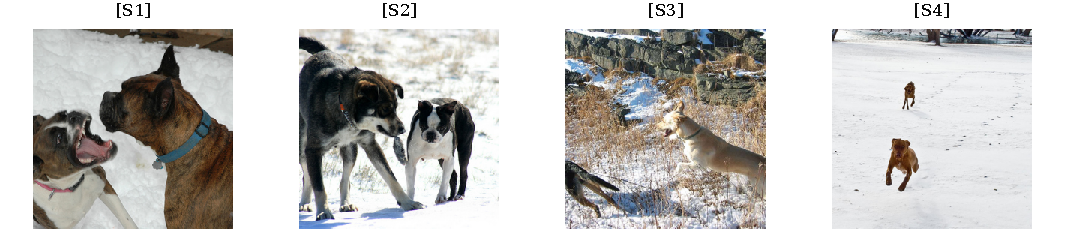
\includegraphics[width=0.92\textwidth]{figures/qualitative.pdf}
\caption{Top-4 results of the full pipeline (SigLIP, hybrid + rerank) for ``two dogs playing in the snow''.
The VLM answer cites them as [S1]--[S4].}
\label{fig:qual}
\end{figure*}

\section{Discussion and Limitations}
\textbf{Cost.} Captioning is done once per image at indexing time and is the most expensive offline step
(Florence-2 detailed captions are the slowest). At query time BGE adds one small text encoding, and reranking
adds 16 passes of a text transformer over cached image features. BLIP-2 is heavier (a 1B-parameter ViT-g,
2.8\,GB of GPU memory in half precision); rescoring all 80K query--candidate pairs took about 25 minutes
in the throttled mode, or about 0.13\,s per query (16 candidates) when the pauses are removed.

\textbf{Cost of v2.} Detection runs once per image at indexing time (Florence-2 \texttt{<OD>}), and the region crops
add about \TBD{X} vectors per image to the index. At query time v2 adds one BLIP-2 ITC text encoding and a
max-pooled search over the region vectors; CB-Norm adds one subtraction per score. The ensemble triples the
dual-encoder cost of stage~1, and a CV-selected pool of $K$ candidates costs $K$ ITM passes.
% TODO(GPU run): put the measured live latency here (results/tables/flickr1k_multi_*_online_v2.md).

\textbf{Scope of evaluation.} The quantitative study covers text\RA image and image\RA text retrieval on
Flickr30k 1K; the larger COCO 5K benchmark is evaluated for text\RA image only, with one encoder and a sample
of 1000 queries. Image + text queries (query fusion with $\beta$) are supported and demonstrated,
but not measured, because Flickr30k has no composed queries; a benchmark such as CIRR would be needed. The
online evaluation uses a 1000-query sample.

\textbf{Possible data overlap.} Both rerankers were fine-tuned on COCO, not Flickr30k, so the COCO 5K evaluation is
in-domain for them. We cannot rule out that
the large pre-training corpora of the captioners and encoders contain Flickr images, which applies equally
to all compared methods.

\textbf{Transductive methods.} Normalising over the whole set of test queries (dual softmax) can raise R@1 but
uses information a real system does not have at query time. We report it only as a labelled ablation
(Table~\ref{tab:v2abl}); CB-Norm, which is part of our system, uses generated captions of the gallery only.

\textbf{No training.} All gains come from combining frozen models. Learning the fusion weights or a small
fusion network on the Flickr30k training split, or fine-tuning the encoders, would likely improve the first
stage and is left for future work.

\balance
\section{Conclusion}
We built a multimodal RAG system around a unified vector database and studied visual-textual feature fusion
for cross-modal retrieval. Fusing an image with a single short caption gives only small gains. Fusion
becomes effective when (i)~captions are detailed and several caption sets are averaged, (ii)~text is compared
with text in a dedicated embedding space and combined with the image score, and (iii)~a cross-attention model
reranks a small, high-recall candidate set. Together these raise Flickr30k 1K text\RA image R@1 from
58.8--74.6 to 84.9--85.9 across three dual encoders without any training, and to 88.3--88.6 with a BLIP-2
reranker, close to task-specific vision-language models evaluated under the same protocol. The live system
reproduces these numbers end to end. On MS-COCO 5K the same stages keep their order but the absolute numbers
are lower (52.2 R@1 for hybrid fusion, 67.3 with BLIP-2), because the larger, more crowded gallery leaves many
similar candidates that only the cross-attention reranker can separate.
v2 adds region and object evidence, a BLIP-2 contrastive channel, caption-bank hubness normalisation and an
encoder ensemble, all without training, and reaches \TBD{XX.X} R@1 on Flickr30k 1K and \TBD{XX.X} on COCO 5K.
% TODO(GPU run): one sentence on which component mattered most, from Table~\ref{tab:v2chain} and Table~\ref{tab:v2abl}.

\begin{thebibliography}{00}
\bibitem{lewis2020rag} P. Lewis \emph{et al.}, ``Retrieval-augmented generation for knowledge-intensive NLP
tasks,'' in \emph{Proc. NeurIPS}, 2020.
\bibitem{chen2022murag} W. Chen, H. Hu, X. Chen, P. Verga, and W. W. Cohen, ``MuRAG: Multimodal
retrieval-augmented generator for open question answering over images and text,'' in \emph{Proc. EMNLP},
2022.
\bibitem{radford2021clip} A. Radford \emph{et al.}, ``Learning transferable visual models from natural
language supervision,'' in \emph{Proc. ICML}, 2021.
\bibitem{zhai2023siglip} X. Zhai, B. Mustafa, A. Kolesnikov, and L. Beyer, ``Sigmoid loss for language
image pre-training,'' in \emph{Proc. ICCV}, 2023.
\bibitem{liang2022gap} W. Liang, Y. Zhang, Y. Kwon, S. Yeung, and J. Zou, ``Mind the gap: Understanding the
modality gap in multi-modal contrastive representation learning,'' in \emph{Proc. NeurIPS}, 2022.
\bibitem{johnson2019faiss} J. Johnson, M. Douze, and H. J\'egou, ``Billion-scale similarity search with
GPUs,'' \emph{IEEE Trans. Big Data}, vol. 7, no. 3, pp. 535--547, 2021.
\bibitem{li2022blip} J. Li, D. Li, C. Xiong, and S. Hoi, ``BLIP: Bootstrapping language-image pre-training
for unified vision-language understanding and generation,'' in \emph{Proc. ICML}, 2022.
\bibitem{xiao2024florence} B. Xiao \emph{et al.}, ``Florence-2: Advancing a unified representation for a
variety of vision tasks,'' in \emph{Proc. CVPR}, 2024.
\bibitem{snoek2005fusion} C. G. M. Snoek, M. Worring, and A. W. M. Smeulders, ``Early versus late fusion in
semantic video analysis,'' in \emph{Proc. ACM Multimedia}, 2005.
\bibitem{cormack2009rrf} G. V. Cormack, C. L. A. Clarke, and S. B\"uttcher, ``Reciprocal rank fusion
outperforms Condorcet and individual rank learning methods,'' in \emph{Proc. SIGIR}, 2009.
\bibitem{li2021albef} J. Li \emph{et al.}, ``Align before fuse: Vision and language representation learning
with momentum distillation,'' in \emph{Proc. NeurIPS}, 2021.
\bibitem{xiao2023bge} S. Xiao, Z. Liu, P. Zhang, and N. Muennighoff, ``C-Pack: Packaged resources to advance
general Chinese embedding,'' arXiv:2309.07597, 2023.
\bibitem{lin2014coco} T.-Y. Lin \emph{et al.}, ``Microsoft COCO: Common objects in context,'' in
\emph{Proc. ECCV}, 2014.
\bibitem{young2014flickr} P. Young, A. Lai, M. Hodosh, and J. Hockenmaier, ``From image descriptions to
visual denotations: New similarity metrics for semantic inference over event descriptions,''
\emph{Trans. ACL}, vol. 2, pp. 67--78, 2014.
\bibitem{karpathy2015deep} A. Karpathy and L. Fei-Fei, ``Deep visual-semantic alignments for generating
image descriptions,'' in \emph{Proc. CVPR}, 2015.
\bibitem{li2023blip2} J. Li, D. Li, S. Savarese, and S. Hoi, ``BLIP-2: Bootstrapping language-image
pre-training with frozen image encoders and large language models,'' in \emph{Proc. ICML}, 2023.
\bibitem{jia2021align} C. Jia \emph{et al.}, ``Scaling up visual and vision-language representation learning
with noisy text supervision,'' in \emph{Proc. ICML}, 2021.
\bibitem{wang2023beit3} W. Wang \emph{et al.}, ``Image as a foreign language: BEiT pretraining for vision and
vision-language tasks,'' in \emph{Proc. CVPR}, 2023.
\bibitem{anderson2018bottomup} P. Anderson \emph{et al.}, ``Bottom-up and top-down attention for image captioning
and visual question answering,'' in \emph{Proc. CVPR}, 2018.
\bibitem{lee2018scan} K.-H. Lee, X. Chen, G. Hua, H. Hu, and X. He, ``Stacked cross attention for image-text
matching,'' in \emph{Proc. ECCV}, 2018.
\bibitem{li2020oscar} X. Li \emph{et al.}, ``Oscar: Object-semantics aligned pre-training for vision-language
tasks,'' in \emph{Proc. ECCV}, 2020.
\bibitem{radovanovic2010hubs} M. Radovanovi\'c, A. Nanopoulos, and M. Ivanovi\'c, ``Hubs in space: Popular nearest
neighbors in high-dimensional data,'' \emph{J. Mach. Learn. Res.}, vol. 11, pp. 2487--2531, 2010.
\bibitem{smith2017invsoftmax} S. L. Smith, D. H. P. Turban, S. Hamblin, and N. Y. Hammerla, ``Offline bilingual word
vectors, orthogonal transformations and the inverted softmax,'' in \emph{Proc. ICLR}, 2017.
\bibitem{bogolin2022qbnorm} S.-V. Bogolin, I. Croitoru, H. Jin, Y. Liu, and S. Albanie, ``Cross modal retrieval with
querybank normalisation,'' in \emph{Proc. CVPR}, 2022.
\bibitem{cheng2021camoe} X. Cheng, H. Lin, X. Wu, F. Yang, and D. Shen, ``Improving video-text retrieval by
multi-stream corpus alignment and dual softmax loss,'' arXiv:2109.04290, 2021.
\bibitem{efron1993bootstrap} B. Efron and R. J. Tibshirani, \emph{An Introduction to the Bootstrap}. Chapman \&
Hall, 1993.
\end{thebibliography}

\end{document}
